\documentclass{standalone}
\usepackage{tikz}
\usetikzlibrary{patterns, positioning}
\usepackage[sfdefault]{ClearSans} %% option 'sfdefault' activates Clear Sans as the default text font
\usepackage[T1]{fontenc}

\begin{document}
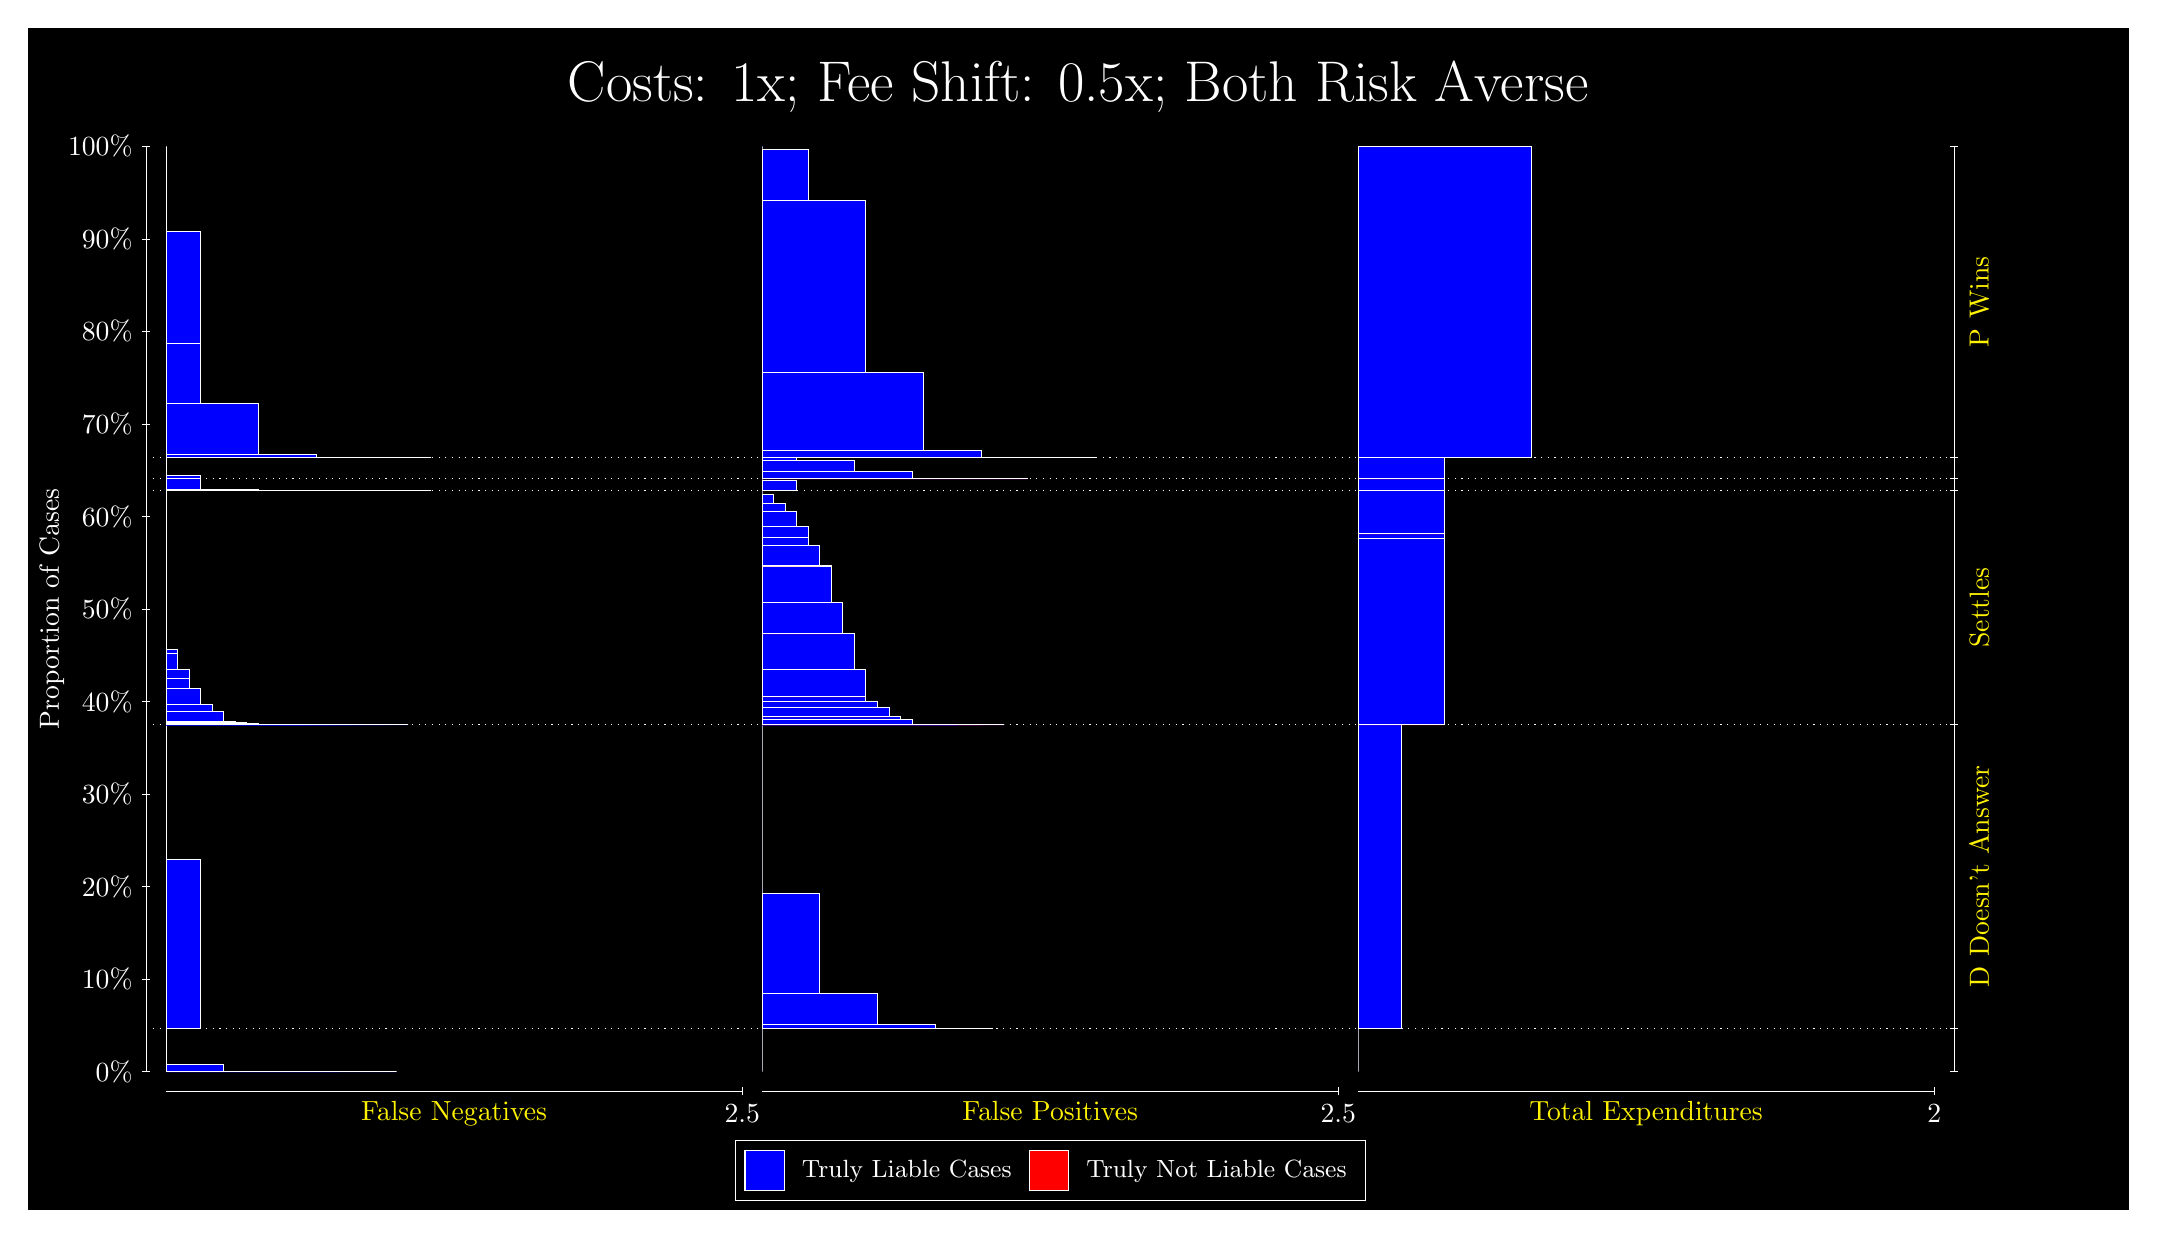
\begin{tikzpicture}
\draw[fill=black] (0,0) rectangle (26.667,15);
\draw[text=white] (0,13.5) rectangle (26.667,15) node[midway] {\huge Costs: 1x; Fee Shift: 0.5x; Both Risk Averse};
\draw[white, very thin] (1.5,1.75) -- (1.5,13.5);
\node[rotate=90, text=white, anchor=center] at (0.3, 7.625) {Proportion of Cases};
\draw[white, very thin] (1.45,1.75) -- (1.55,1.75);
\node[text=white, anchor=east] at (1.45, 1.75) {0\%};
\draw[white, very thin] (1.45,2.925) -- (1.55,2.925);
\node[text=white, anchor=east] at (1.45, 2.925) {10\%};
\draw[white, very thin] (1.45,4.1) -- (1.55,4.1);
\node[text=white, anchor=east] at (1.45, 4.1) {20\%};
\draw[white, very thin] (1.45,5.275) -- (1.55,5.275);
\node[text=white, anchor=east] at (1.45, 5.275) {30\%};
\draw[white, very thin] (1.45,6.45) -- (1.55,6.45);
\node[text=white, anchor=east] at (1.45, 6.45) {40\%};
\draw[white, very thin] (1.45,7.625) -- (1.55,7.625);
\node[text=white, anchor=east] at (1.45, 7.625) {50\%};
\draw[white, very thin] (1.45,8.8) -- (1.55,8.8);
\node[text=white, anchor=east] at (1.45, 8.8) {60\%};
\draw[white, very thin] (1.45,9.975) -- (1.55,9.975);
\node[text=white, anchor=east] at (1.45, 9.975) {70\%};
\draw[white, very thin] (1.45,11.15) -- (1.55,11.15);
\node[text=white, anchor=east] at (1.45, 11.15) {80\%};
\draw[white, very thin] (1.45,12.325) -- (1.55,12.325);
\node[text=white, anchor=east] at (1.45, 12.325) {90\%};
\draw[white, very thin] (1.45,13.5) -- (1.55,13.5);
\node[text=white, anchor=east] at (1.45, 13.5) {100\%};

\draw[white, very thin] (24.457,1.75) -- (24.457,13.5);
\draw[white, very thin] (24.407,1.75) -- (24.507,1.75);
\node[anchor=west] at (24.407, 1.75) {};
\draw[white, very thin] (24.407,2.2986) -- (24.507,2.2986);
\node[anchor=west] at (24.407, 2.2986) {};
\draw[white, very thin] (24.407,6.1566) -- (24.507,6.1566);
\node[anchor=west] at (24.407, 6.1566) {};
\draw[white, very thin] (24.407,9.1305) -- (24.507,9.1305);
\node[anchor=west] at (24.407, 9.1305) {};
\draw[white, very thin] (24.407,9.2804) -- (24.507,9.2804);
\node[anchor=west] at (24.407, 9.2804) {};
\draw[white, very thin] (24.407,9.5513) -- (24.507,9.5513);
\node[anchor=west] at (24.407, 9.5513) {};
\draw[white, very thin] (24.407,13.5) -- (24.507,13.5);
\node[anchor=west] at (24.407, 13.5) {};

\draw[white, very thin, fill=blue] (1.75,1.75) rectangle (4.6775,1.75);
\draw[white, very thin, fill=blue] (1.75,1.75) rectangle (3.9457,1.75);
\draw[white, very thin, fill=blue] (1.75,1.75) rectangle (3.2138,1.7508);
\draw[white, very thin, fill=blue] (1.75,1.7508) rectangle (2.4819,1.8398);
\draw[white, very thin, fill=red] (1.75,1.8398) rectangle (1.75,1.8398);
\draw[white, very thin, fill=blue] (1.75,1.8398) rectangle (1.75,2.2986);
\draw[white, very thin, fill=blue] (1.75,2.2986) rectangle (2.1891,4.4395);
\draw[white, very thin, fill=red] (1.75,4.4395) rectangle (1.75,4.4395);
\draw[white, very thin, fill=blue] (1.75,4.4395) rectangle (1.75,6.1566);
\draw[white, very thin, fill=blue] (1.75,6.1566) rectangle (4.8239,6.1566);
\draw[white, very thin, fill=blue] (1.75,6.1566) rectangle (4.5312,6.1566);
\draw[white, very thin, fill=blue] (1.75,6.1566) rectangle (4.2384,6.1566);
\draw[white, very thin, fill=blue] (1.75,6.1566) rectangle (4.092,6.1566);
\draw[white, very thin, fill=blue] (1.75,6.1566) rectangle (3.9457,6.1566);
\draw[white, very thin, fill=blue] (1.75,6.1566) rectangle (3.7993,6.1566);
\draw[white, very thin, fill=blue] (1.75,6.1566) rectangle (3.6529,6.1566);
\draw[white, very thin, fill=blue] (1.75,6.1566) rectangle (3.5065,6.1567);
\draw[white, very thin, fill=blue] (1.75,6.1567) rectangle (3.3602,6.1567);
\draw[white, very thin, fill=blue] (1.75,6.1567) rectangle (3.2138,6.1567);
\draw[white, very thin, fill=blue] (1.75,6.1567) rectangle (3.0674,6.1583);
\draw[white, very thin, fill=blue] (1.75,6.1583) rectangle (3.0674,6.1583);
\draw[white, very thin, fill=blue] (1.75,6.1583) rectangle (2.921,6.1668);
\draw[white, very thin, fill=blue] (1.75,6.1668) rectangle (2.7746,6.1831);
\draw[white, very thin, fill=blue] (1.75,6.1831) rectangle (2.6283,6.1949);
\draw[white, very thin, fill=blue] (1.75,6.1949) rectangle (2.6283,6.2003);
\draw[white, very thin, fill=blue] (1.75,6.2003) rectangle (2.4819,6.3217);
\draw[white, very thin, fill=blue] (1.75,6.3217) rectangle (2.3355,6.412);
\draw[white, very thin, fill=blue] (1.75,6.412) rectangle (2.3355,6.4169);
\draw[white, very thin, fill=blue] (1.75,6.4169) rectangle (2.1891,6.6123);
\draw[white, very thin, fill=blue] (1.75,6.6123) rectangle (2.0428,6.7467);
\draw[white, very thin, fill=blue] (1.75,6.7467) rectangle (2.0428,6.8551);
\draw[white, very thin, fill=blue] (1.75,6.8551) rectangle (1.8964,7.0636);
\draw[white, very thin, fill=blue] (1.75,7.0636) rectangle (1.8964,7.1138);
\draw[white, very thin, fill=blue] (1.75,7.1138) rectangle (1.75,7.1152);
\draw[white, very thin, fill=red] (1.75,7.1152) rectangle (1.75,7.1152);
\draw[white, very thin, fill=blue] (1.75,7.1152) rectangle (1.75,9.1305);
\draw[white, very thin, fill=blue] (1.75,9.1305) rectangle (5.1167,9.1305);
\draw[white, very thin, fill=blue] (1.75,9.1305) rectangle (4.3848,9.1305);
\draw[white, very thin, fill=blue] (1.75,9.1305) rectangle (3.6529,9.1306);
\draw[white, very thin, fill=blue] (1.75,9.1306) rectangle (2.921,9.1503);
\draw[white, very thin, fill=blue] (1.75,9.1503) rectangle (2.1891,9.2804);
\draw[white, very thin, fill=red] (1.75,9.2804) rectangle (1.75,9.2804);
\draw[white, very thin, fill=blue] (1.75,9.2804) rectangle (2.1891,9.3191);
\draw[white, very thin, fill=red] (1.75,9.3191) rectangle (1.75,9.3191);
\draw[white, very thin, fill=blue] (1.75,9.3191) rectangle (1.75,9.5513);
\draw[white, very thin, fill=blue] (1.75,9.5513) rectangle (5.1167,9.5513);
\draw[white, very thin, fill=blue] (1.75,9.5513) rectangle (4.3848,9.5515);
\draw[white, very thin, fill=blue] (1.75,9.5515) rectangle (3.6529,9.5857);
\draw[white, very thin, fill=blue] (1.75,9.5857) rectangle (2.921,10.239);
\draw[white, very thin, fill=blue] (1.75,10.239) rectangle (2.1891,10.997);
\draw[white, very thin, fill=blue] (1.75,10.997) rectangle (2.1891,12.42);
\draw[white, very thin, fill=red] (1.75,12.42) rectangle (1.75,12.42);
\draw[white, very thin, fill=blue] (1.75,12.42) rectangle (1.75,13.5);
\draw[white, very thin, fill=red] (9.3189,1.75) rectangle (9.3189,1.75);
\draw[white, very thin, fill=blue] (9.3189,1.75) rectangle (9.3189,2.2986);
\draw[white, very thin, fill=red] (9.3189,2.2986) rectangle (12.246,2.2986);
\draw[white, very thin, fill=blue] (9.3189,2.2986) rectangle (12.246,2.299);
\draw[white, very thin, fill=blue] (9.3189,2.299) rectangle (11.515,2.3451);
\draw[white, very thin, fill=blue] (9.3189,2.3451) rectangle (10.783,2.7453);
\draw[white, very thin, fill=blue] (9.3189,2.7453) rectangle (10.051,4.0158);
\draw[white, very thin, fill=blue] (9.3189,4.0158) rectangle (9.3189,6.1566);
\draw[white, very thin, fill=red] (9.3189,6.1566) rectangle (12.393,6.1566);
\draw[white, very thin, fill=blue] (9.3189,6.1566) rectangle (12.393,6.1566);
\draw[white, very thin, fill=red] (9.3189,6.1566) rectangle (12.1,6.1566);
\draw[white, very thin, fill=blue] (9.3189,6.1566) rectangle (12.1,6.1566);
\draw[white, very thin, fill=red] (9.3189,6.1566) rectangle (11.807,6.1566);
\draw[white, very thin, fill=blue] (9.3189,6.1566) rectangle (11.807,6.1568);
\draw[white, very thin, fill=blue] (9.3189,6.1568) rectangle (11.661,6.1583);
\draw[white, very thin, fill=red] (9.3189,6.1583) rectangle (11.515,6.1583);
\draw[white, very thin, fill=blue] (9.3189,6.1583) rectangle (11.515,6.1588);
\draw[white, very thin, fill=blue] (9.3189,6.1588) rectangle (11.368,6.1609);
\draw[white, very thin, fill=red] (9.3189,6.1609) rectangle (11.222,6.1609);
\draw[white, very thin, fill=blue] (9.3189,6.1609) rectangle (11.222,6.224);
\draw[white, very thin, fill=blue] (9.3189,6.224) rectangle (11.075,6.257);
\draw[white, very thin, fill=red] (9.3189,6.257) rectangle (10.929,6.257);
\draw[white, very thin, fill=blue] (9.3189,6.257) rectangle (10.929,6.3744);
\draw[white, very thin, fill=red] (9.3189,6.3744) rectangle (10.929,6.3744);
\draw[white, very thin, fill=blue] (9.3189,6.3744) rectangle (10.929,6.3744);
\draw[white, very thin, fill=blue] (9.3189,6.3744) rectangle (10.783,6.4514);
\draw[white, very thin, fill=blue] (9.3189,6.4514) rectangle (10.636,6.5101);
\draw[white, very thin, fill=red] (9.3189,6.5101) rectangle (10.636,6.5101);
\draw[white, very thin, fill=blue] (9.3189,6.5101) rectangle (10.636,6.8642);
\draw[white, very thin, fill=blue] (9.3189,6.8642) rectangle (10.49,7.3104);
\draw[white, very thin, fill=red] (9.3189,7.3104) rectangle (10.344,7.3104);
\draw[white, very thin, fill=blue] (9.3189,7.3104) rectangle (10.344,7.7038);
\draw[white, very thin, fill=blue] (9.3189,7.7038) rectangle (10.197,8.1718);
\draw[white, very thin, fill=blue] (9.3189,8.1718) rectangle (10.197,8.1732);
\draw[white, very thin, fill=red] (9.3189,8.1732) rectangle (10.051,8.1732);
\draw[white, very thin, fill=blue] (9.3189,8.1732) rectangle (10.051,8.432);
\draw[white, very thin, fill=blue] (9.3189,8.432) rectangle (9.9044,8.5404);
\draw[white, very thin, fill=blue] (9.3189,8.5404) rectangle (9.9044,8.6747);
\draw[white, very thin, fill=blue] (9.3189,8.6747) rectangle (9.758,8.8702);
\draw[white, very thin, fill=blue] (9.3189,8.8702) rectangle (9.6116,8.9654);
\draw[white, very thin, fill=blue] (9.3189,8.9654) rectangle (9.4652,9.0867);
\draw[white, very thin, fill=blue] (9.3189,9.0867) rectangle (9.4652,9.0868);
\draw[white, very thin, fill=blue] (9.3189,9.0868) rectangle (9.3189,9.1305);
\draw[white, very thin, fill=red] (9.3189,9.1305) rectangle (9.758,9.1305);
\draw[white, very thin, fill=blue] (9.3189,9.1305) rectangle (9.758,9.2606);
\draw[white, very thin, fill=blue] (9.3189,9.2606) rectangle (9.3189,9.2804);
\draw[white, very thin, fill=red] (9.3189,9.2804) rectangle (12.686,9.2804);
\draw[white, very thin, fill=blue] (9.3189,9.2804) rectangle (12.686,9.2805);
\draw[white, very thin, fill=blue] (9.3189,9.2805) rectangle (11.954,9.2895);
\draw[white, very thin, fill=blue] (9.3189,9.2895) rectangle (11.222,9.3674);
\draw[white, very thin, fill=blue] (9.3189,9.3674) rectangle (10.49,9.5126);
\draw[white, very thin, fill=blue] (9.3189,9.5126) rectangle (9.758,9.5513);
\draw[white, very thin, fill=red] (9.3189,9.5513) rectangle (13.564,9.5513);
\draw[white, very thin, fill=blue] (9.3189,9.5513) rectangle (13.564,9.5513);
\draw[white, very thin, fill=red] (9.3189,9.5513) rectangle (12.832,9.5513);
\draw[white, very thin, fill=blue] (9.3189,9.5513) rectangle (12.832,9.5525);
\draw[white, very thin, fill=red] (9.3189,9.5525) rectangle (12.1,9.5525);
\draw[white, very thin, fill=blue] (9.3189,9.5525) rectangle (12.1,9.6387);
\draw[white, very thin, fill=red] (9.3189,9.6387) rectangle (11.368,9.6387);
\draw[white, very thin, fill=blue] (9.3189,9.6387) rectangle (11.368,10.631);
\draw[white, very thin, fill=red] (9.3189,10.631) rectangle (10.636,10.631);
\draw[white, very thin, fill=blue] (9.3189,10.631) rectangle (10.636,12.813);
\draw[white, very thin, fill=blue] (9.3189,12.813) rectangle (9.9044,13.466);
\draw[white, very thin, fill=blue] (9.3189,13.466) rectangle (9.3189,13.5);
\draw[white, very thin, fill=red] (16.888,1.75) rectangle (16.888,1.75);
\draw[white, very thin, fill=blue] (16.888,1.75) rectangle (16.888,2.2986);
\draw[white, very thin, fill=red] (16.888,2.2986) rectangle (17.437,2.2986);
\draw[white, very thin, fill=blue] (16.888,2.2986) rectangle (17.437,6.1566);
\draw[white, very thin, fill=red] (16.888,6.1566) rectangle (17.986,6.1566);
\draw[white, very thin, fill=blue] (16.888,6.1566) rectangle (17.986,8.527);
\draw[white, very thin, fill=red] (16.888,8.527) rectangle (17.986,8.527);
\draw[white, very thin, fill=blue] (16.888,8.527) rectangle (17.986,8.5825);
\draw[white, very thin, fill=red] (16.888,8.5825) rectangle (17.986,8.5825);
\draw[white, very thin, fill=blue] (16.888,8.5825) rectangle (17.986,9.1305);
\draw[white, very thin, fill=red] (16.888,9.1305) rectangle (17.986,9.1305);
\draw[white, very thin, fill=blue] (16.888,9.1305) rectangle (17.986,9.2804);
\draw[white, very thin, fill=red] (16.888,9.2804) rectangle (17.986,9.2804);
\draw[white, very thin, fill=blue] (16.888,9.2804) rectangle (17.986,9.5513);
\draw[white, very thin, fill=red] (16.888,9.5513) rectangle (19.083,9.5513);
\draw[white, very thin, fill=blue] (16.888,9.5513) rectangle (19.083,13.5);
\draw[white, dotted] (1.5,2.2986) -- (24.457,2.2986);
\draw[white, dotted] (1.5,6.1566) -- (24.457,6.1566);
\draw[white, dotted] (1.5,9.1305) -- (24.457,9.1305);
\draw[white, dotted] (1.5,9.2804) -- (24.457,9.2804);
\draw[white, dotted] (1.5,9.5513) -- (24.457,9.5513);
\draw[white, very thin] (1.75,1.5) -- (9.0689,1.5);
\node[text=yellow, anchor=north] at (5.4094, 1.5) {False Negatives};
\draw[white, very thin] (9.0689,1.45) -- (9.0689,1.55);
\node[text=white, anchor=north] at (9.0689, 1.45) {2.5};

\draw[white, very thin] (9.3189,1.5) -- (16.638,1.5);
\node[text=yellow, anchor=north] at (12.978, 1.5) {False Positives};
\draw[white, very thin] (16.638,1.45) -- (16.638,1.55);
\node[text=white, anchor=north] at (16.638, 1.45) {2.5};

\draw[white, very thin] (16.888,1.5) -- (24.207,1.5);
\node[text=yellow, anchor=north] at (20.547, 1.5) {Total Expenditures};
\draw[white, very thin] (24.207,1.45) -- (24.207,1.55);
\node[text=white, anchor=north] at (24.207, 1.45) {2};


\node[text=yellow, centered, rotate=90] at (24.777, 4.2276) {D Doesn't Answer};
\node[text=yellow, centered, rotate=90] at (24.777, 7.6435) {Settles};


\node[text=yellow, centered, rotate=90] at (24.777, 11.526) {P Wins};

\draw (12.978300999999998,1.5) node[draw=none] (baseCoordinate) {};
\begin{scope}[align=center]
        \matrix[scale=0.5, draw=white, below=0.5cm of baseCoordinate, nodes={draw}, column sep=0.1cm]{
            \node[rectangle, draw, minimum width=0.5cm, minimum height=0.5cm, fill=blue] {}; &
            \node[draw=none, font=\small, text=white] (B) {Truly Liable Cases}; &
            \node[rectangle, draw, minimum width=0.5cm, minimum height=0.5cm, fill=red] {}; &
            \node[draw=none, font=\small, text=white] (B) {Truly Not Liable Cases}; \\
            };
\end{scope}

\end{tikzpicture}
\end{document}